\documentclass[11pt]{article}
\usepackage{latexsym}
\usepackage{natbib}
\usepackage{graphicx}
\usepackage{caption}
\usepackage{subcaption}
\usepackage{listings}
\usepackage{algorithm}
\usepackage{algpseudocode}

\title{Homework 4: Approximate Inference in Bayesian Networks}
\author{Shun Zhang}
\date{}

\begin{document}
\maketitle

\section{Sampling Methods}

In this assignment, I implemented Rejection Sampling and Gibbs
Sampling to generate samples for a Bayesian network. 

For Rejection Sampling, the implementation is quite simple. Samples
are generated ignoring the constraints of the evidence. Then, samples
inconsistent with the evidence are dropped. In the remaining samples,
proportion of samples consistent with the query is returned.

For Gibbs Sampling, in each iteration, for node $x_i$, it is sampled
from the following probability (revised from the textbook).

\begin{equation}
p(x_i|x_{\{j \not = i\}}) \propto \prod_k P(x_k|pa_k)
\end{equation}

\section{Experiments}

\begin{figure}
\centering
\begin{subfigure}[b]{0.49\textwidth}
	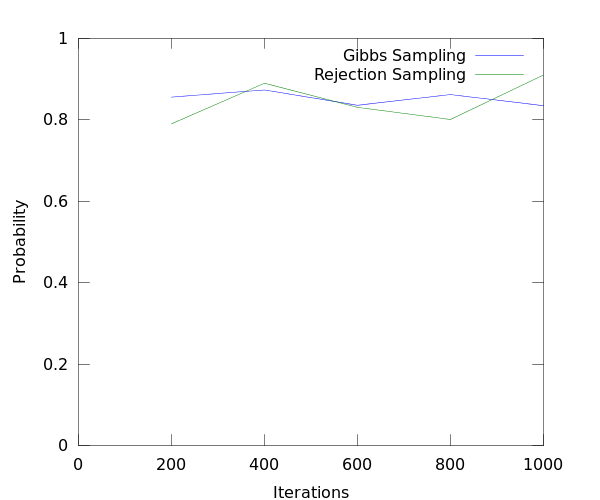
\includegraphics[width=\textwidth]{ian1.png}
	\caption{$P(X_0=1 | E_1) $}
	\end{subfigure}
\begin{subfigure}[b]{0.49\textwidth}
	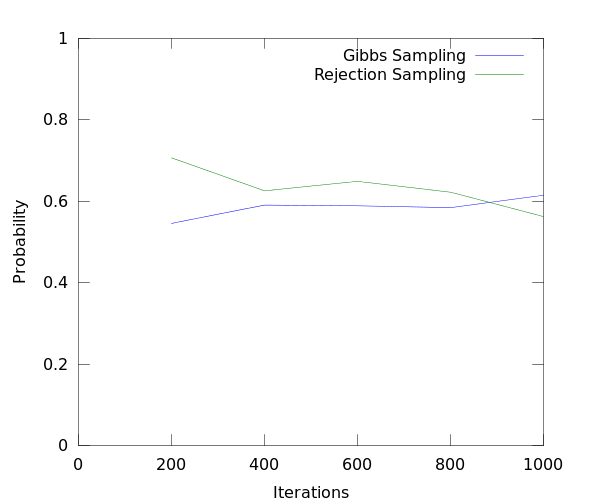
\includegraphics[width=\textwidth]{ian2.png}
	\caption{$P(X_1=1 | E_1) $}
\end{subfigure}
\begin{subfigure}[b]{0.49\textwidth}
	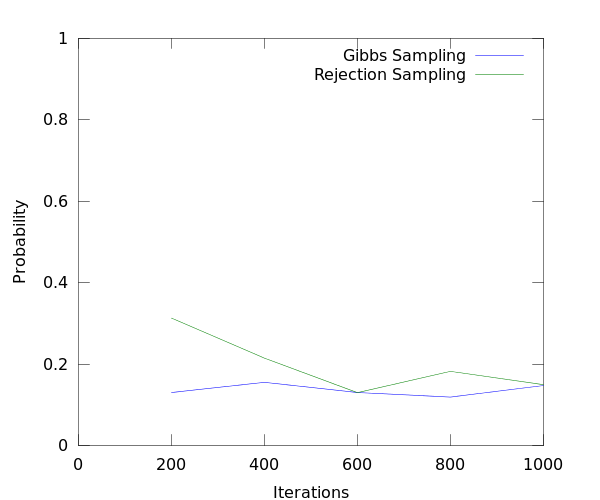
\includegraphics[width=\textwidth]{ian3.png}
	\caption{$P(X_2=1 | E_1) $}
\end{subfigure}
\begin{subfigure}[b]{0.49\textwidth}
	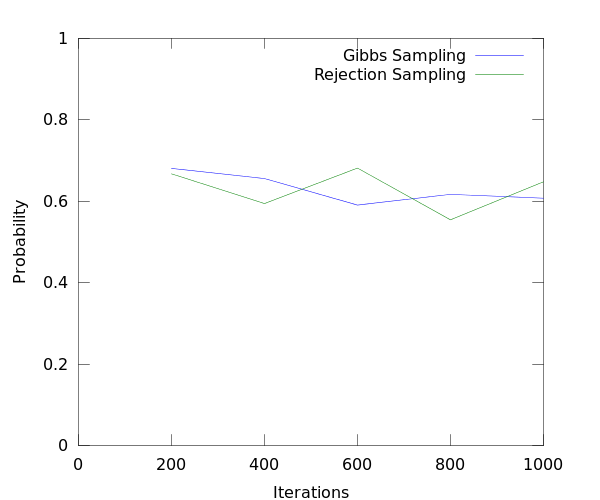
\includegraphics[width=\textwidth]{ian4.png}
	\caption{$P(X_3=1 | E_1) $}
\end{subfigure}
\begin{subfigure}[b]{0.49\textwidth}
	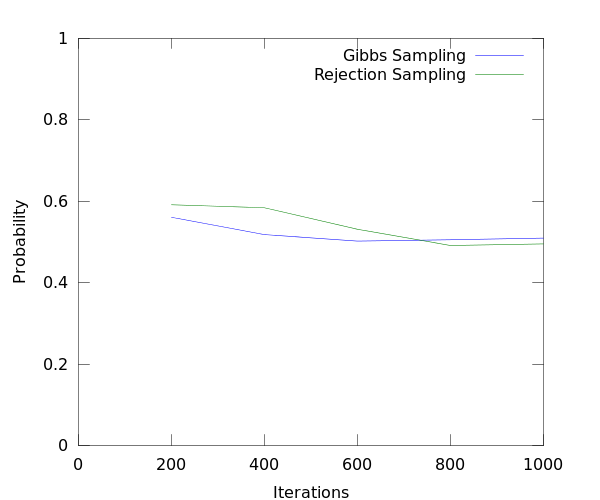
\includegraphics[width=\textwidth]{ian5.png}
	\caption{$P(X_4=1 | E_1) $}
\end{subfigure}
\begin{subfigure}[b]{0.49\textwidth}
	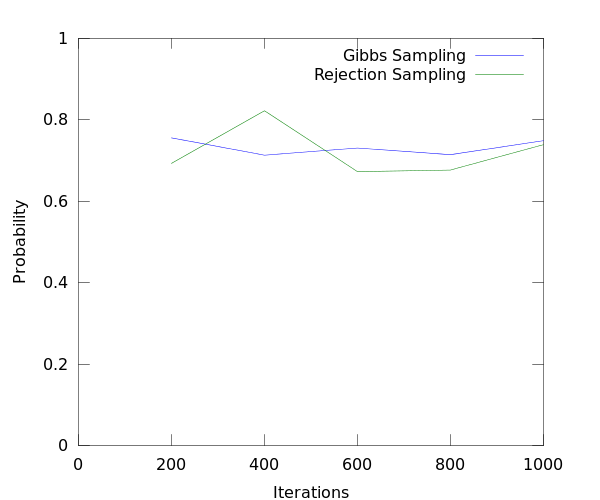
\includegraphics[width=\textwidth]{ian6.png}
	\caption{$P(X_5=1 | E_1) $}
\end{subfigure}
\caption{Sampling process for each test case. $E_1$ denotes $(X_6 = 1,
X_7 = 0, X_8 = 0)$.}
\label{fig:lp}
\end{figure}

In this experiment, I used the data provided by Ian. The running
iterations for both are 1000. Note for rejection sampling, the samples
collected are less than 1000. For Gibbs sampling, the parameter $T =
200$. The algorithm starts collect data after $T$ iteraions. The
results generated are shown below.

In Figure~\ref{fig:lp}, I show the learning process in each sampling
algorithms, for each query data for the first envidence given.

\begin{samepage}
The following is the numerical results. Each line corresponds to one
evidence. Each number is the result of one query. They are ordered as
given.

By rejection sampling,

\begin{verbatim}
   0.848837   0.538462   0.142857   0.638298   0.607143   0.750000
   0.795082   0.766129   0.132231   0.990566   0.393939   0.170213
   0.862069   0.642857   0.134021   0.515789   0.450000   0.240385
   0.831579   0.644689   0.130268   0.944649   0.350195   0.847059
   0.930000   0.715909   0.098901   0.495050   0.403670   0.282828
   0.828125   0.648649   0.094595   1.000000   0.742857   0.810811
   0.849462   0.571429   0.122449   0.394737   0.554348   0.611111
   0.825688   0.791304   0.148515   0.943925   0.333333   0.111111
   0.773585   0.696203   0.109091   0.964912   0.731707   0.745098
   0.855263   0.533333   0.117155   0.519824   0.427928   0.836538
\end{verbatim}

By Gibbs sampling,

\begin{verbatim}
   0.83500    0.56800    0.13300    0.62500    0.49600    0.75200
   0.81700    0.77600    0.11900    0.95500    0.38800    0.16700
   0.84900    0.68200    0.12400    0.44900    0.44000    0.29100
   0.81500    0.64300    0.13300    0.96700    0.35700    0.86100
   0.84500    0.65900    0.12900    0.49500    0.46700    0.27800
   0.82600    0.66100    0.15900    0.97600    0.76700    0.68700
   0.85200    0.59900    0.13800    0.42300    0.54600    0.65200
   0.78800    0.79200    0.10800    0.96300    0.35200    0.15000
   0.81600    0.66100    0.13100    0.97800    0.76800    0.72400
   0.87300    0.51800    0.12000    0.54100    0.41800    0.82000
\end{verbatim}
\end{samepage}

\section{Discussion}

The rejection sampling is less efficient in general, because it
generates samples inconsistent with the evidence. This depends on the
probability of the evidence - if the evidence is very unlikely, then
the algorithm needs to run many times to gather enough samples
consistent with the evidence.

In this sense, Gibbs sampling beats rejection sampling because every
sample counts. However, Gibbs sampling relies on the initial sample in
the first few iterations. It needs some iterations to reach a
stationary distribution.

\end{document}
